\documentclass{standalone}
\usepackage{tikz}
\usetikzlibrary{patterns, positioning}

\begin{document}
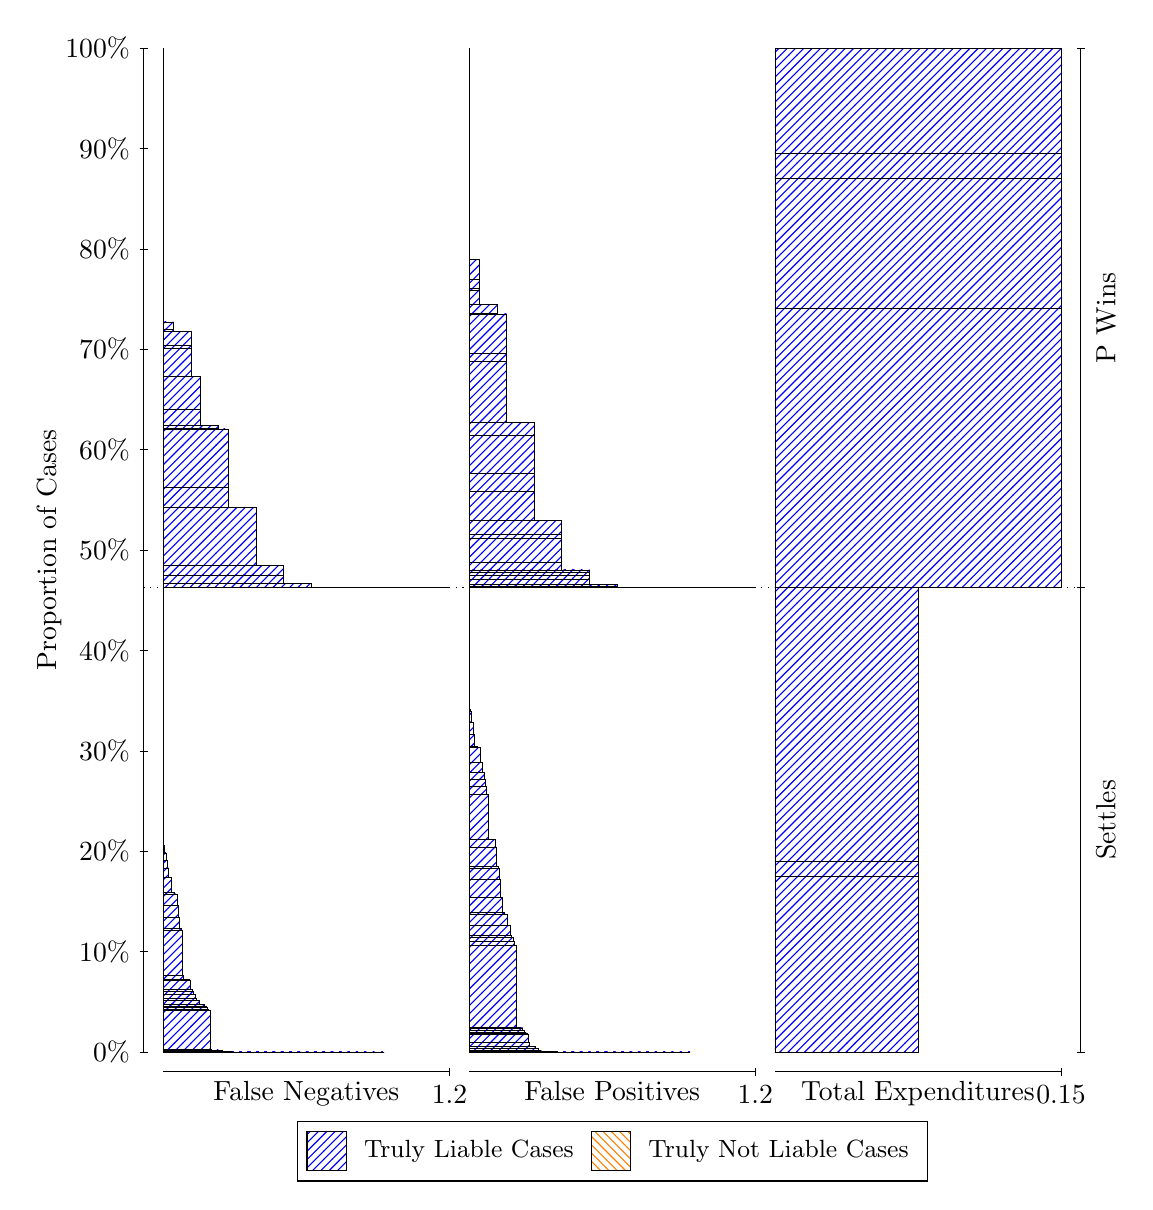
\begin{tikzpicture}
\draw[black, very thin] (1.5,1.75) -- (1.5,14.5);
\node[rotate=90, anchor=center] at (0.3, 8.125) {Proportion of Cases};
\draw[black, very thin] (1.45,1.75) -- (1.55,1.75);
\node[anchor=east] at (1.45, 1.75) {0\%};
\draw[black, very thin] (1.45,3.025) -- (1.55,3.025);
\node[anchor=east] at (1.45, 3.025) {10\%};
\draw[black, very thin] (1.45,4.3) -- (1.55,4.3);
\node[anchor=east] at (1.45, 4.3) {20\%};
\draw[black, very thin] (1.45,5.575) -- (1.55,5.575);
\node[anchor=east] at (1.45, 5.575) {30\%};
\draw[black, very thin] (1.45,6.85) -- (1.55,6.85);
\node[anchor=east] at (1.45, 6.85) {40\%};
\draw[black, very thin] (1.45,8.125) -- (1.55,8.125);
\node[anchor=east] at (1.45, 8.125) {50\%};
\draw[black, very thin] (1.45,9.4) -- (1.55,9.4);
\node[anchor=east] at (1.45, 9.4) {60\%};
\draw[black, very thin] (1.45,10.675) -- (1.55,10.675);
\node[anchor=east] at (1.45, 10.675) {70\%};
\draw[black, very thin] (1.45,11.95) -- (1.55,11.95);
\node[anchor=east] at (1.45, 11.95) {80\%};
\draw[black, very thin] (1.45,13.225) -- (1.55,13.225);
\node[anchor=east] at (1.45, 13.225) {90\%};
\draw[black, very thin] (1.45,14.5) -- (1.55,14.5);
\node[anchor=east] at (1.45, 14.5) {100\%};

\draw[black, very thin] (13.4,1.75) -- (13.4,14.5);
\draw[black, very thin] (13.35,1.75) -- (13.45,1.75);
\node[anchor=west] at (13.35, 1.75) {};
\draw[black, very thin] (13.35,7.6465) -- (13.45,7.6465);
\node[anchor=west] at (13.35, 7.6465) {};
\draw[black, very thin] (13.35,14.5) -- (13.45,14.5);
\node[anchor=west] at (13.35, 14.5) {};

\draw[black, very thin, pattern color=blue, pattern=north east lines] (1.75,1.75) rectangle (4.554,1.75);
\draw[black, very thin, pattern color=blue, pattern=north east lines] (1.75,1.75) rectangle (4.396,1.75);
\draw[black, very thin, pattern color=blue, pattern=north east lines] (1.75,1.75) rectangle (4.238,1.75);
\draw[black, very thin, pattern color=blue, pattern=north east lines] (1.75,1.75) rectangle (4.2029,1.75);
\draw[black, very thin, pattern color=blue, pattern=north east lines] (1.75,1.75) rectangle (4.0801,1.75);
\draw[black, very thin, pattern color=blue, pattern=north east lines] (1.75,1.75) rectangle (4.045,1.75);
\draw[black, very thin, pattern color=blue, pattern=north east lines] (1.75,1.75) rectangle (3.9221,1.75);
\draw[black, very thin, pattern color=blue, pattern=north east lines] (1.75,1.75) rectangle (3.887,1.75);
\draw[black, very thin, pattern color=blue, pattern=north east lines] (1.75,1.75) rectangle (3.8519,1.75);
\draw[black, very thin, pattern color=blue, pattern=north east lines] (1.75,1.75) rectangle (3.7641,1.75);
\draw[black, very thin, pattern color=blue, pattern=north east lines] (1.75,1.75) rectangle (3.729,1.75);
\draw[black, very thin, pattern color=blue, pattern=north east lines] (1.75,1.75) rectangle (3.6939,1.75);
\draw[black, very thin, pattern color=blue, pattern=north east lines] (1.75,1.75) rectangle (3.6062,1.75);
\draw[black, very thin, pattern color=blue, pattern=north east lines] (1.75,1.75) rectangle (3.5711,1.75);
\draw[black, very thin, pattern color=blue, pattern=north east lines] (1.75,1.75) rectangle (3.536,1.75);
\draw[black, very thin, pattern color=blue, pattern=north east lines] (1.75,1.75) rectangle (3.5008,1.75);
\draw[black, very thin, pattern color=blue, pattern=north east lines] (1.75,1.75) rectangle (3.4482,1.75);
\draw[black, very thin, pattern color=blue, pattern=north east lines] (1.75,1.75) rectangle (3.4131,1.75);
\draw[black, very thin, pattern color=blue, pattern=north east lines] (1.75,1.75) rectangle (3.378,1.75);
\draw[black, very thin, pattern color=blue, pattern=north east lines] (1.75,1.75) rectangle (3.3429,1.75);
\draw[black, very thin, pattern color=blue, pattern=north east lines] (1.75,1.75) rectangle (3.2902,1.75);
\draw[black, very thin, pattern color=blue, pattern=north east lines] (1.75,1.75) rectangle (3.2551,1.75);
\draw[black, very thin, pattern color=blue, pattern=north east lines] (1.75,1.75) rectangle (3.22,1.75);
\draw[black, very thin, pattern color=blue, pattern=north east lines] (1.75,1.75) rectangle (3.1849,1.75);
\draw[black, very thin, pattern color=blue, pattern=north east lines] (1.75,1.75) rectangle (3.1498,1.75);
\draw[black, very thin, pattern color=blue, pattern=north east lines] (1.75,1.75) rectangle (3.1322,1.75);
\draw[black, very thin, pattern color=blue, pattern=north east lines] (1.75,1.75) rectangle (3.0971,1.75);
\draw[black, very thin, pattern color=blue, pattern=north east lines] (1.75,1.75) rectangle (3.062,1.75);
\draw[black, very thin, pattern color=blue, pattern=north east lines] (1.75,1.75) rectangle (3.0269,1.75);
\draw[black, very thin, pattern color=blue, pattern=north east lines] (1.75,1.75) rectangle (2.9918,1.75);
\draw[black, very thin, pattern color=blue, pattern=north east lines] (1.75,1.75) rectangle (2.9743,1.75);
\draw[black, very thin, pattern color=blue, pattern=north east lines] (1.75,1.75) rectangle (2.9392,1.75);
\draw[black, very thin, pattern color=blue, pattern=north east lines] (1.75,1.75) rectangle (2.9041,1.75);
\draw[black, very thin, pattern color=blue, pattern=north east lines] (1.75,1.75) rectangle (2.869,1.75);
\draw[black, very thin, pattern color=blue, pattern=north east lines] (1.75,1.75) rectangle (2.8339,1.75);
\draw[black, very thin, pattern color=blue, pattern=north east lines] (1.75,1.75) rectangle (2.8163,1.7501);
\draw[black, very thin, pattern color=blue, pattern=north east lines] (1.75,1.7501) rectangle (2.7988,1.7501);
\draw[black, very thin, pattern color=blue, pattern=north east lines] (1.75,1.7501) rectangle (2.7812,1.7501);
\draw[black, very thin, pattern color=blue, pattern=north east lines] (1.75,1.7501) rectangle (2.7461,1.7501);
\draw[black, very thin, pattern color=blue, pattern=north east lines] (1.75,1.7501) rectangle (2.711,1.7502);
\draw[black, very thin, pattern color=blue, pattern=north east lines] (1.75,1.7502) rectangle (2.6759,1.7504);
\draw[black, very thin, pattern color=blue, pattern=north east lines] (1.75,1.7504) rectangle (2.6583,1.7518);
\draw[black, very thin, pattern color=blue, pattern=north east lines] (1.75,1.7518) rectangle (2.6408,1.7522);
\draw[black, very thin, pattern color=blue, pattern=north east lines] (1.75,1.7522) rectangle (2.6232,1.7528);
\draw[black, very thin, pattern color=blue, pattern=north east lines] (1.75,1.7528) rectangle (2.5881,1.7529);
\draw[black, very thin, pattern color=blue, pattern=north east lines] (1.75,1.7529) rectangle (2.553,1.7552);
\draw[black, very thin, pattern color=blue, pattern=north east lines] (1.75,1.7552) rectangle (2.5179,1.7556);
\draw[black, very thin, pattern color=blue, pattern=north east lines] (1.75,1.7556) rectangle (2.5004,1.7656);
\draw[black, very thin, pattern color=blue, pattern=north east lines] (1.75,1.7656) rectangle (2.4828,1.7675);
\draw[black, very thin, pattern color=blue, pattern=north east lines] (1.75,1.7675) rectangle (2.4653,1.7697);
\draw[black, very thin, pattern color=blue, pattern=north east lines] (1.75,1.7697) rectangle (2.4477,1.7754);
\draw[black, very thin, pattern color=blue, pattern=north east lines] (1.75,1.7754) rectangle (2.4302,1.7755);
\draw[black, very thin, pattern color=blue, pattern=north east lines] (1.75,1.7755) rectangle (2.395,1.7756);
\draw[black, very thin, pattern color=blue, pattern=north east lines] (1.75,1.7756) rectangle (2.3599,1.7804);
\draw[black, very thin, pattern color=blue, pattern=north east lines] (1.75,1.7804) rectangle (2.3424,2.284);
\draw[black, very thin, pattern color=blue, pattern=north east lines] (1.75,2.284) rectangle (2.3248,2.289);
\draw[black, very thin, pattern color=blue, pattern=north east lines] (1.75,2.289) rectangle (2.3073,2.3161);
\draw[black, very thin, pattern color=blue, pattern=north east lines] (1.75,2.3161) rectangle (2.2897,2.3366);
\draw[black, very thin, pattern color=blue, pattern=north east lines] (1.75,2.3366) rectangle (2.2722,2.3575);
\draw[black, very thin, pattern color=blue, pattern=north east lines] (1.75,2.3575) rectangle (2.2371,2.3605);
\draw[black, very thin, pattern color=blue, pattern=north east lines] (1.75,2.3605) rectangle (2.202,2.4088);
\draw[black, very thin, pattern color=blue, pattern=north east lines] (1.75,2.4088) rectangle (2.1669,2.4275);
\draw[black, very thin, pattern color=blue, pattern=north east lines] (1.75,2.4275) rectangle (2.1493,2.4829);
\draw[black, very thin, pattern color=blue, pattern=north east lines] (1.75,2.4829) rectangle (2.1318,2.5154);
\draw[black, very thin, pattern color=blue, pattern=north east lines] (1.75,2.5154) rectangle (2.1142,2.5483);
\draw[black, very thin, pattern color=blue, pattern=north east lines] (1.75,2.5483) rectangle (2.0967,2.6663);
\draw[black, very thin, pattern color=blue, pattern=north east lines] (1.75,2.6663) rectangle (2.0791,2.6682);
\draw[black, very thin, pattern color=blue, pattern=north east lines] (1.75,2.6682) rectangle (2.044,2.67);
\draw[black, very thin, pattern color=blue, pattern=north east lines] (1.75,2.67) rectangle (2.0089,2.7188);
\draw[black, very thin, pattern color=blue, pattern=north east lines] (1.75,2.7188) rectangle (1.9913,3.2901);
\draw[black, very thin, pattern color=blue, pattern=north east lines] (1.75,3.2901) rectangle (1.9738,3.3157);
\draw[black, very thin, pattern color=blue, pattern=north east lines] (1.75,3.3157) rectangle (1.9562,3.4612);
\draw[black, very thin, pattern color=blue, pattern=north east lines] (1.75,3.4612) rectangle (1.9387,3.6107);
\draw[black, very thin, pattern color=blue, pattern=north east lines] (1.75,3.6107) rectangle (1.9211,3.7588);
\draw[black, very thin, pattern color=blue, pattern=north east lines] (1.75,3.7588) rectangle (1.886,3.778);
\draw[black, very thin, pattern color=blue, pattern=north east lines] (1.75,3.778) rectangle (1.8509,3.9706);
\draw[black, very thin, pattern color=blue, pattern=north east lines] (1.75,3.9706) rectangle (1.8158,4.0886);
\draw[black, very thin, pattern color=blue, pattern=north east lines] (1.75,4.0886) rectangle (1.7983,4.183);
\draw[black, very thin, pattern color=blue, pattern=north east lines] (1.75,4.183) rectangle (1.7807,4.2773);
\draw[black, very thin, pattern color=blue, pattern=north east lines] (1.75,4.2773) rectangle (1.7632,4.3705);
\draw[black, very thin, pattern color=orange, pattern=north west lines] (1.75,4.3705) rectangle (1.75,4.3705);
\draw[black, very thin, pattern color=blue, pattern=north east lines] (1.75,4.3705) rectangle (1.75,7.6465);
\draw[black, very thin, pattern color=blue, pattern=north east lines] (1.75,7.6465) rectangle (5.3833,7.6465);
\draw[black, very thin, pattern color=blue, pattern=north east lines] (1.75,7.6465) rectangle (5.0323,7.6465);
\draw[black, very thin, pattern color=blue, pattern=north east lines] (1.75,7.6465) rectangle (5.0323,7.6465);
\draw[black, very thin, pattern color=blue, pattern=north east lines] (1.75,7.6465) rectangle (4.6812,7.6465);
\draw[black, very thin, pattern color=blue, pattern=north east lines] (1.75,7.6465) rectangle (4.6812,7.6465);
\draw[black, very thin, pattern color=blue, pattern=north east lines] (1.75,7.6465) rectangle (4.3302,7.6469);
\draw[black, very thin, pattern color=blue, pattern=north east lines] (1.75,7.6469) rectangle (4.2073,7.6469);
\draw[black, very thin, pattern color=blue, pattern=north east lines] (1.75,7.6469) rectangle (3.9791,7.6505);
\draw[black, very thin, pattern color=blue, pattern=north east lines] (1.75,7.6505) rectangle (3.9791,7.6524);
\draw[black, very thin, pattern color=blue, pattern=north east lines] (1.75,7.6524) rectangle (3.8563,7.6524);
\draw[black, very thin, pattern color=blue, pattern=north east lines] (1.75,7.6524) rectangle (3.8563,7.6524);
\draw[black, very thin, pattern color=blue, pattern=north east lines] (1.75,7.6524) rectangle (3.6281,7.6982);
\draw[black, very thin, pattern color=blue, pattern=north east lines] (1.75,7.6982) rectangle (3.5052,7.6982);
\draw[black, very thin, pattern color=blue, pattern=north east lines] (1.75,7.6982) rectangle (3.2771,7.8079);
\draw[black, very thin, pattern color=blue, pattern=north east lines] (1.75,7.8079) rectangle (3.2771,7.934);
\draw[black, very thin, pattern color=blue, pattern=north east lines] (1.75,7.934) rectangle (3.1542,7.934);
\draw[black, very thin, pattern color=blue, pattern=north east lines] (1.75,7.934) rectangle (3.1542,7.934);
\draw[black, very thin, pattern color=blue, pattern=north east lines] (1.75,7.934) rectangle (2.926,8.6626);
\draw[black, very thin, pattern color=blue, pattern=north east lines] (1.75,8.6626) rectangle (2.8031,8.6633);
\draw[black, very thin, pattern color=blue, pattern=north east lines] (1.75,8.6633) rectangle (2.8031,8.6633);
\draw[black, very thin, pattern color=blue, pattern=north east lines] (1.75,8.6633) rectangle (2.8031,8.6637);
\draw[black, very thin, pattern color=blue, pattern=north east lines] (1.75,8.6637) rectangle (2.575,8.922);
\draw[black, very thin, pattern color=blue, pattern=north east lines] (1.75,8.922) rectangle (2.575,9.6637);
\draw[black, very thin, pattern color=blue, pattern=north east lines] (1.75,9.6637) rectangle (2.4521,9.6646);
\draw[black, very thin, pattern color=blue, pattern=north east lines] (1.75,9.6646) rectangle (2.4521,9.7098);
\draw[black, very thin, pattern color=blue, pattern=north east lines] (1.75,9.7098) rectangle (2.2239,9.913);
\draw[black, very thin, pattern color=blue, pattern=north east lines] (1.75,9.913) rectangle (2.2239,10.329);
\draw[black, very thin, pattern color=blue, pattern=north east lines] (1.75,10.329) rectangle (2.101,10.684);
\draw[black, very thin, pattern color=blue, pattern=north east lines] (1.75,10.684) rectangle (2.101,10.719);
\draw[black, very thin, pattern color=blue, pattern=north east lines] (1.75,10.719) rectangle (2.101,10.902);
\draw[black, very thin, pattern color=blue, pattern=north east lines] (1.75,10.902) rectangle (1.8729,10.903);
\draw[black, very thin, pattern color=blue, pattern=north east lines] (1.75,10.903) rectangle (1.8729,10.928);
\draw[black, very thin, pattern color=blue, pattern=north east lines] (1.75,10.928) rectangle (1.8729,11.02);
\draw[black, very thin, pattern color=blue, pattern=north east lines] (1.75,11.02) rectangle (1.8729,11.022);
\draw[black, very thin, pattern color=orange, pattern=north west lines] (1.75,11.022) rectangle (1.75,11.022);
\draw[black, very thin, pattern color=blue, pattern=north east lines] (1.75,11.022) rectangle (1.75,14.5);
\draw[black, very thin, pattern color=orange, pattern=north west lines] (5.6333,1.75) rectangle (8.4373,1.75);
\draw[black, very thin, pattern color=blue, pattern=north east lines] (5.6333,1.75) rectangle (8.4373,1.75);
\draw[black, very thin, pattern color=orange, pattern=north west lines] (5.6333,1.75) rectangle (8.2793,1.75);
\draw[black, very thin, pattern color=blue, pattern=north east lines] (5.6333,1.75) rectangle (8.2793,1.75);
\draw[black, very thin, pattern color=orange, pattern=north west lines] (5.6333,1.75) rectangle (8.1214,1.75);
\draw[black, very thin, pattern color=blue, pattern=north east lines] (5.6333,1.75) rectangle (8.1214,1.75);
\draw[black, very thin, pattern color=blue, pattern=north east lines] (5.6333,1.75) rectangle (8.0863,1.75);
\draw[black, very thin, pattern color=orange, pattern=north west lines] (5.6333,1.75) rectangle (7.9634,1.75);
\draw[black, very thin, pattern color=blue, pattern=north east lines] (5.6333,1.75) rectangle (7.9634,1.75);
\draw[black, very thin, pattern color=blue, pattern=north east lines] (5.6333,1.75) rectangle (7.9283,1.75);
\draw[black, very thin, pattern color=orange, pattern=north west lines] (5.6333,1.75) rectangle (7.8054,1.75);
\draw[black, very thin, pattern color=blue, pattern=north east lines] (5.6333,1.75) rectangle (7.8054,1.75);
\draw[black, very thin, pattern color=blue, pattern=north east lines] (5.6333,1.75) rectangle (7.7703,1.75);
\draw[black, very thin, pattern color=blue, pattern=north east lines] (5.6333,1.75) rectangle (7.7352,1.75);
\draw[black, very thin, pattern color=orange, pattern=north west lines] (5.6333,1.75) rectangle (7.6475,1.75);
\draw[black, very thin, pattern color=blue, pattern=north east lines] (5.6333,1.75) rectangle (7.6475,1.75);
\draw[black, very thin, pattern color=blue, pattern=north east lines] (5.6333,1.75) rectangle (7.6124,1.75);
\draw[black, very thin, pattern color=blue, pattern=north east lines] (5.6333,1.75) rectangle (7.5773,1.75);
\draw[black, very thin, pattern color=orange, pattern=north west lines] (5.6333,1.75) rectangle (7.4895,1.75);
\draw[black, very thin, pattern color=blue, pattern=north east lines] (5.6333,1.75) rectangle (7.4895,1.75);
\draw[black, very thin, pattern color=blue, pattern=north east lines] (5.6333,1.75) rectangle (7.4544,1.75);
\draw[black, very thin, pattern color=blue, pattern=north east lines] (5.6333,1.75) rectangle (7.4193,1.75);
\draw[black, very thin, pattern color=blue, pattern=north east lines] (5.6333,1.75) rectangle (7.3842,1.75);
\draw[black, very thin, pattern color=orange, pattern=north west lines] (5.6333,1.75) rectangle (7.3315,1.75);
\draw[black, very thin, pattern color=blue, pattern=north east lines] (5.6333,1.75) rectangle (7.3315,1.75);
\draw[black, very thin, pattern color=blue, pattern=north east lines] (5.6333,1.75) rectangle (7.2964,1.75);
\draw[black, very thin, pattern color=blue, pattern=north east lines] (5.6333,1.75) rectangle (7.2613,1.75);
\draw[black, very thin, pattern color=blue, pattern=north east lines] (5.6333,1.75) rectangle (7.2262,1.75);
\draw[black, very thin, pattern color=orange, pattern=north west lines] (5.6333,1.75) rectangle (7.1736,1.75);
\draw[black, very thin, pattern color=blue, pattern=north east lines] (5.6333,1.75) rectangle (7.1736,1.75);
\draw[black, very thin, pattern color=blue, pattern=north east lines] (5.6333,1.75) rectangle (7.1384,1.75);
\draw[black, very thin, pattern color=blue, pattern=north east lines] (5.6333,1.75) rectangle (7.1033,1.75);
\draw[black, very thin, pattern color=blue, pattern=north east lines] (5.6333,1.75) rectangle (7.0682,1.75);
\draw[black, very thin, pattern color=blue, pattern=north east lines] (5.6333,1.75) rectangle (7.0331,1.75);
\draw[black, very thin, pattern color=orange, pattern=north west lines] (5.6333,1.75) rectangle (7.0156,1.75);
\draw[black, very thin, pattern color=blue, pattern=north east lines] (5.6333,1.75) rectangle (7.0156,1.7501);
\draw[black, very thin, pattern color=blue, pattern=north east lines] (5.6333,1.7501) rectangle (6.9805,1.7501);
\draw[black, very thin, pattern color=blue, pattern=north east lines] (5.6333,1.7501) rectangle (6.9454,1.7501);
\draw[black, very thin, pattern color=blue, pattern=north east lines] (5.6333,1.7501) rectangle (6.9103,1.7502);
\draw[black, very thin, pattern color=blue, pattern=north east lines] (5.6333,1.7502) rectangle (6.8752,1.7502);
\draw[black, very thin, pattern color=orange, pattern=north west lines] (5.6333,1.7502) rectangle (6.8576,1.7502);
\draw[black, very thin, pattern color=blue, pattern=north east lines] (5.6333,1.7502) rectangle (6.8576,1.7511);
\draw[black, very thin, pattern color=blue, pattern=north east lines] (5.6333,1.7511) rectangle (6.8225,1.7517);
\draw[black, very thin, pattern color=blue, pattern=north east lines] (5.6333,1.7517) rectangle (6.7874,1.7518);
\draw[black, very thin, pattern color=blue, pattern=north east lines] (5.6333,1.7518) rectangle (6.7523,1.7541);
\draw[black, very thin, pattern color=blue, pattern=north east lines] (5.6333,1.7541) rectangle (6.7172,1.7547);
\draw[black, very thin, pattern color=orange, pattern=north west lines] (5.6333,1.7547) rectangle (6.6996,1.7547);
\draw[black, very thin, pattern color=blue, pattern=north east lines] (5.6333,1.7547) rectangle (6.6996,1.7551);
\draw[black, very thin, pattern color=blue, pattern=north east lines] (5.6333,1.7551) rectangle (6.6821,1.7556);
\draw[black, very thin, pattern color=blue, pattern=north east lines] (5.6333,1.7556) rectangle (6.6645,1.7578);
\draw[black, very thin, pattern color=blue, pattern=north east lines] (5.6333,1.7578) rectangle (6.6294,1.7579);
\draw[black, very thin, pattern color=blue, pattern=north east lines] (5.6333,1.7579) rectangle (6.5943,1.7581);
\draw[black, very thin, pattern color=blue, pattern=north east lines] (5.6333,1.7581) rectangle (6.5592,1.7628);
\draw[black, very thin, pattern color=orange, pattern=north west lines] (5.6333,1.7628) rectangle (6.5417,1.7628);
\draw[black, very thin, pattern color=blue, pattern=north east lines] (5.6333,1.7628) rectangle (6.5417,1.7728);
\draw[black, very thin, pattern color=blue, pattern=north east lines] (5.6333,1.7728) rectangle (6.5241,1.7747);
\draw[black, very thin, pattern color=blue, pattern=north east lines] (5.6333,1.7747) rectangle (6.5066,1.7961);
\draw[black, very thin, pattern color=blue, pattern=north east lines] (5.6333,1.7961) rectangle (6.4715,1.8169);
\draw[black, very thin, pattern color=blue, pattern=north east lines] (5.6333,1.8169) rectangle (6.4364,1.8199);
\draw[black, very thin, pattern color=blue, pattern=north east lines] (5.6333,1.8199) rectangle (6.4012,1.8682);
\draw[black, very thin, pattern color=orange, pattern=north west lines] (5.6333,1.8682) rectangle (6.3837,1.8682);
\draw[black, very thin, pattern color=blue, pattern=north east lines] (5.6333,1.8682) rectangle (6.3837,1.9692);
\draw[black, very thin, pattern color=blue, pattern=north east lines] (5.6333,1.9692) rectangle (6.3661,1.9928);
\draw[black, very thin, pattern color=blue, pattern=north east lines] (5.6333,1.9928) rectangle (6.3486,1.9985);
\draw[black, very thin, pattern color=blue, pattern=north east lines] (5.6333,1.9985) rectangle (6.331,2.0241);
\draw[black, very thin, pattern color=blue, pattern=north east lines] (5.6333,2.0241) rectangle (6.3135,2.0571);
\draw[black, very thin, pattern color=blue, pattern=north east lines] (5.6333,2.0571) rectangle (6.2784,2.059);
\draw[black, very thin, pattern color=blue, pattern=north east lines] (5.6333,2.059) rectangle (6.2433,2.0608);
\draw[black, very thin, pattern color=orange, pattern=north west lines] (5.6333,2.0608) rectangle (6.2257,2.0608);
\draw[black, very thin, pattern color=blue, pattern=north east lines] (5.6333,2.0608) rectangle (6.2257,3.1014);
\draw[black, very thin, pattern color=blue, pattern=north east lines] (5.6333,3.1014) rectangle (6.2082,3.1496);
\draw[black, very thin, pattern color=blue, pattern=north east lines] (5.6333,3.1496) rectangle (6.1906,3.205);
\draw[black, very thin, pattern color=blue, pattern=north east lines] (5.6333,3.205) rectangle (6.1731,3.2376);
\draw[black, very thin, pattern color=blue, pattern=north east lines] (5.6333,3.2376) rectangle (6.1555,3.3571);
\draw[black, very thin, pattern color=blue, pattern=north east lines] (5.6333,3.3571) rectangle (6.1204,3.5048);
\draw[black, very thin, pattern color=blue, pattern=north east lines] (5.6333,3.5048) rectangle (6.0853,3.5239);
\draw[black, very thin, pattern color=blue, pattern=north east lines] (5.6333,3.5239) rectangle (6.0502,3.7169);
\draw[black, very thin, pattern color=blue, pattern=north east lines] (5.6333,3.7169) rectangle (6.0326,3.938);
\draw[black, very thin, pattern color=blue, pattern=north east lines] (5.6333,3.938) rectangle (6.0151,4.0817);
\draw[black, very thin, pattern color=blue, pattern=north east lines] (5.6333,4.0817) rectangle (5.9975,4.1077);
\draw[black, very thin, pattern color=blue, pattern=north east lines] (5.6333,4.1077) rectangle (5.98,4.3515);
\draw[black, very thin, pattern color=blue, pattern=north east lines] (5.6333,4.3515) rectangle (5.9624,4.4452);
\draw[black, very thin, pattern color=blue, pattern=north east lines] (5.6333,4.4452) rectangle (5.9273,4.4499);
\draw[black, very thin, pattern color=blue, pattern=north east lines] (5.6333,4.4499) rectangle (5.8922,4.4547);
\draw[black, very thin, pattern color=blue, pattern=north east lines] (5.6333,4.4547) rectangle (5.8747,5.0259);
\draw[black, very thin, pattern color=blue, pattern=north east lines] (5.6333,5.0259) rectangle (5.8571,5.1192);
\draw[black, very thin, pattern color=blue, pattern=north east lines] (5.6333,5.1192) rectangle (5.8396,5.2135);
\draw[black, very thin, pattern color=blue, pattern=north east lines] (5.6333,5.2135) rectangle (5.822,5.3078);
\draw[black, very thin, pattern color=blue, pattern=north east lines] (5.6333,5.3078) rectangle (5.8045,5.4259);
\draw[black, very thin, pattern color=blue, pattern=north east lines] (5.6333,5.4259) rectangle (5.7694,5.6185);
\draw[black, very thin, pattern color=blue, pattern=north east lines] (5.6333,5.6185) rectangle (5.7343,5.6376);
\draw[black, very thin, pattern color=blue, pattern=north east lines] (5.6333,5.6376) rectangle (5.6992,5.7858);
\draw[black, very thin, pattern color=blue, pattern=north east lines] (5.6333,5.7858) rectangle (5.6816,5.9353);
\draw[black, very thin, pattern color=blue, pattern=north east lines] (5.6333,5.9353) rectangle (5.664,6.0807);
\draw[black, very thin, pattern color=blue, pattern=north east lines] (5.6333,6.0807) rectangle (5.6465,6.1064);
\draw[black, very thin, pattern color=blue, pattern=north east lines] (5.6333,6.1064) rectangle (5.6333,7.6465);
\draw[black, very thin, pattern color=orange, pattern=north west lines] (5.6333,7.6465) rectangle (9.2667,7.6465);
\draw[black, very thin, pattern color=blue, pattern=north east lines] (5.6333,7.6465) rectangle (9.2667,7.6465);
\draw[black, very thin, pattern color=orange, pattern=north west lines] (5.6333,7.6465) rectangle (8.9156,7.6465);
\draw[black, very thin, pattern color=blue, pattern=north east lines] (5.6333,7.6465) rectangle (8.9156,7.6465);
\draw[black, very thin, pattern color=orange, pattern=north west lines] (5.6333,7.6465) rectangle (8.5646,7.6465);
\draw[black, very thin, pattern color=blue, pattern=north east lines] (5.6333,7.6465) rectangle (8.5646,7.6465);
\draw[black, very thin, pattern color=blue, pattern=north east lines] (5.6333,7.6465) rectangle (8.5646,7.6465);
\draw[black, very thin, pattern color=blue, pattern=north east lines] (5.6333,7.6465) rectangle (8.5646,7.6465);
\draw[black, very thin, pattern color=orange, pattern=north west lines] (5.6333,7.6465) rectangle (8.2135,7.6465);
\draw[black, very thin, pattern color=blue, pattern=north east lines] (5.6333,7.6465) rectangle (8.2135,7.6467);
\draw[black, very thin, pattern color=blue, pattern=north east lines] (5.6333,7.6467) rectangle (8.2135,7.6467);
\draw[black, very thin, pattern color=orange, pattern=north west lines] (5.6333,7.6467) rectangle (8.0907,7.6467);
\draw[black, very thin, pattern color=blue, pattern=north east lines] (5.6333,7.6467) rectangle (8.0907,7.6467);
\draw[black, very thin, pattern color=orange, pattern=north west lines] (5.6333,7.6467) rectangle (7.8625,7.6467);
\draw[black, very thin, pattern color=blue, pattern=north east lines] (5.6333,7.6467) rectangle (7.8625,7.6479);
\draw[black, very thin, pattern color=blue, pattern=north east lines] (5.6333,7.6479) rectangle (7.8625,7.6506);
\draw[black, very thin, pattern color=blue, pattern=north east lines] (5.6333,7.6506) rectangle (7.7396,7.6506);
\draw[black, very thin, pattern color=orange, pattern=north west lines] (5.6333,7.6506) rectangle (7.7396,7.6506);
\draw[black, very thin, pattern color=blue, pattern=north east lines] (5.6333,7.6506) rectangle (7.7396,7.6506);
\draw[black, very thin, pattern color=blue, pattern=north east lines] (5.6333,7.6506) rectangle (7.5114,7.6617);
\draw[black, very thin, pattern color=orange, pattern=north west lines] (5.6333,7.6617) rectangle (7.5114,7.6617);
\draw[black, very thin, pattern color=blue, pattern=north east lines] (5.6333,7.6617) rectangle (7.5114,7.6697);
\draw[black, very thin, pattern color=blue, pattern=north east lines] (5.6333,7.6697) rectangle (7.5114,7.6854);
\draw[black, very thin, pattern color=orange, pattern=north west lines] (5.6333,7.6854) rectangle (7.3886,7.6854);
\draw[black, very thin, pattern color=blue, pattern=north east lines] (5.6333,7.6854) rectangle (7.3886,7.6854);
\draw[black, very thin, pattern color=blue, pattern=north east lines] (5.6333,7.6854) rectangle (7.1604,7.7492);
\draw[black, very thin, pattern color=blue, pattern=north east lines] (5.6333,7.7492) rectangle (7.1604,7.7987);
\draw[black, very thin, pattern color=orange, pattern=north west lines] (5.6333,7.7987) rectangle (7.1604,7.7987);
\draw[black, very thin, pattern color=blue, pattern=north east lines] (5.6333,7.7987) rectangle (7.1604,7.8377);
\draw[black, very thin, pattern color=blue, pattern=north east lines] (5.6333,7.8377) rectangle (7.1604,7.873);
\draw[black, very thin, pattern color=blue, pattern=north east lines] (5.6333,7.873) rectangle (7.0375,7.873);
\draw[black, very thin, pattern color=orange, pattern=north west lines] (5.6333,7.873) rectangle (7.0375,7.873);
\draw[black, very thin, pattern color=blue, pattern=north east lines] (5.6333,7.873) rectangle (7.0375,7.873);
\draw[black, very thin, pattern color=blue, pattern=north east lines] (5.6333,7.873) rectangle (6.8093,7.9652);
\draw[black, very thin, pattern color=orange, pattern=north west lines] (5.6333,7.9652) rectangle (6.8093,7.9652);
\draw[black, very thin, pattern color=blue, pattern=north east lines] (5.6333,7.9652) rectangle (6.8093,8.2733);
\draw[black, very thin, pattern color=blue, pattern=north east lines] (5.6333,8.2733) rectangle (6.8093,8.3249);
\draw[black, very thin, pattern color=blue, pattern=north east lines] (5.6333,8.3249) rectangle (6.8093,8.503);
\draw[black, very thin, pattern color=blue, pattern=north east lines] (5.6333,8.503) rectangle (6.6865,8.503);
\draw[black, very thin, pattern color=orange, pattern=north west lines] (5.6333,8.503) rectangle (6.6865,8.503);
\draw[black, very thin, pattern color=blue, pattern=north east lines] (5.6333,8.503) rectangle (6.6865,8.503);
\draw[black, very thin, pattern color=blue, pattern=north east lines] (5.6333,8.503) rectangle (6.4583,8.8732);
\draw[black, very thin, pattern color=blue, pattern=north east lines] (5.6333,8.8732) rectangle (6.4583,9.0939);
\draw[black, very thin, pattern color=blue, pattern=north east lines] (5.6333,9.0939) rectangle (6.4583,9.5791);
\draw[black, very thin, pattern color=blue, pattern=north east lines] (5.6333,9.5791) rectangle (6.4583,9.7424);
\draw[black, very thin, pattern color=blue, pattern=north east lines] (5.6333,9.7424) rectangle (6.3354,9.7424);
\draw[black, very thin, pattern color=orange, pattern=north west lines] (5.6333,9.7424) rectangle (6.3354,9.7424);
\draw[black, very thin, pattern color=blue, pattern=north east lines] (5.6333,9.7424) rectangle (6.3354,9.7457);
\draw[black, very thin, pattern color=blue, pattern=north east lines] (5.6333,9.7457) rectangle (6.1072,10.521);
\draw[black, very thin, pattern color=blue, pattern=north east lines] (5.6333,10.521) rectangle (6.1072,10.618);
\draw[black, very thin, pattern color=blue, pattern=north east lines] (5.6333,10.618) rectangle (6.1072,11.125);
\draw[black, very thin, pattern color=blue, pattern=north east lines] (5.6333,11.125) rectangle (5.9844,11.126);
\draw[black, very thin, pattern color=orange, pattern=north west lines] (5.6333,11.126) rectangle (5.9844,11.126);
\draw[black, very thin, pattern color=blue, pattern=north east lines] (5.6333,11.126) rectangle (5.9844,11.244);
\draw[black, very thin, pattern color=blue, pattern=north east lines] (5.6333,11.244) rectangle (5.9844,11.245);
\draw[black, very thin, pattern color=blue, pattern=north east lines] (5.6333,11.245) rectangle (5.7562,11.428);
\draw[black, very thin, pattern color=blue, pattern=north east lines] (5.6333,11.428) rectangle (5.7562,11.445);
\draw[black, very thin, pattern color=blue, pattern=north east lines] (5.6333,11.445) rectangle (5.7562,11.563);
\draw[black, very thin, pattern color=blue, pattern=north east lines] (5.6333,11.563) rectangle (5.7562,11.817);
\draw[black, very thin, pattern color=orange, pattern=north west lines] (5.6333,11.817) rectangle (5.6333,11.817);
\draw[black, very thin, pattern color=blue, pattern=north east lines] (5.6333,11.817) rectangle (5.6333,14.5);
\draw[black, very thin, pattern color=orange, pattern=north west lines] (9.5167,1.75) rectangle (11.333,1.75);
\draw[black, very thin, pattern color=blue, pattern=north east lines] (9.5167,1.75) rectangle (11.333,3.978);
\draw[black, very thin, pattern color=orange, pattern=north west lines] (9.5167,3.978) rectangle (11.333,3.978);
\draw[black, very thin, pattern color=blue, pattern=north east lines] (9.5167,3.978) rectangle (11.333,4.1722);
\draw[black, very thin, pattern color=orange, pattern=north west lines] (9.5167,4.1722) rectangle (11.333,4.1722);
\draw[black, very thin, pattern color=blue, pattern=north east lines] (9.5167,4.1722) rectangle (11.333,7.6465);
\draw[black, very thin, pattern color=orange, pattern=north west lines] (9.5167,7.6465) rectangle (13.15,7.6465);
\draw[black, very thin, pattern color=blue, pattern=north east lines] (9.5167,7.6465) rectangle (13.15,11.196);
\draw[black, very thin, pattern color=orange, pattern=north west lines] (9.5167,11.196) rectangle (13.15,11.196);
\draw[black, very thin, pattern color=blue, pattern=north east lines] (9.5167,11.196) rectangle (13.15,12.848);
\draw[black, very thin, pattern color=orange, pattern=north west lines] (9.5167,12.848) rectangle (13.15,12.848);
\draw[black, very thin, pattern color=blue, pattern=north east lines] (9.5167,12.848) rectangle (13.15,13.158);
\draw[black, very thin, pattern color=orange, pattern=north west lines] (9.5167,13.158) rectangle (13.15,13.158);
\draw[black, very thin, pattern color=blue, pattern=north east lines] (9.5167,13.158) rectangle (13.15,14.5);
\draw[black, dotted] (1.5,7.6465) -- (13.4,7.6465);
\draw[black, very thin] (1.75,1.5) -- (5.3833,1.5);
\node[anchor=north] at (3.5667, 1.5) {False Negatives};
\draw[black, very thin] (5.3833,1.45) -- (5.3833,1.55);
\node[anchor=north] at (5.3833, 1.45) {1.2};

\draw[black, very thin] (5.6333,1.5) -- (9.2667,1.5);
\node[anchor=north] at (7.45, 1.5) {False Positives};
\draw[black, very thin] (9.2667,1.45) -- (9.2667,1.55);
\node[anchor=north] at (9.2667, 1.45) {1.2};

\draw[black, very thin] (9.5167,1.5) -- (13.15,1.5);
\node[anchor=north] at (11.333, 1.5) {Total Expenditures};
\draw[black, very thin] (13.15,1.45) -- (13.15,1.55);
\node[anchor=north] at (13.15, 1.45) {0.15};

\node[black, centered, rotate=90] at (13.72, 4.6982) {Settles};
\node[black, centered, rotate=90] at (13.72, 11.073) {P Wins};

\draw (7.449999999999999,1.5) node[draw=none] (baseCoordinate) {};
\begin{scope}[align=center]
        \matrix[scale=0.5, draw=black, below=0.5cm of baseCoordinate, nodes={draw}, column sep=0.1cm]{
            \node[rectangle, draw, minimum width=0.5cm, minimum height=0.5cm, pattern=north east lines, pattern color=blue] {}; &
            \node[draw=none, font=\small] (B) {Truly Liable Cases}; &
            \node[rectangle, draw, minimum width=0.5cm, minimum height=0.5cm, pattern=north west lines, pattern color=orange] {}; &
            \node[draw=none, font=\small] (B) {Truly Not Liable Cases}; \\
            };
\end{scope}

\end{tikzpicture}
\end{document}